\documentclass[10pt,a4paper]{beamer}
\usepackage[utf8]{inputenc}
\usepackage[francais]{babel}
\usepackage[T1]{fontenc}
\usepackage{amsmath}
\usepackage{amsfonts}
\usepackage{amssymb}
\usepackage{graphicx}
\usepackage{lmodern}

\author{Pierre \bsc{Donat-Bouillud} Thibaud \bsc{Ehret}}
\title{Lancer de rayons}

\begin{document}

\section{Organisation générale.}
\begin{frame}
\frametitle{Organisation pratique}
\framesubtitle{150 commits !}
\only<1>{
\begin{block}{Git et github}
	\begin{multicols}{2}
	\begin{itemize}
	\item versions
	\item système « d'issues » de Github
	\item nombreux graphiques pour visualiser l'avancement du travail
	\end{itemize}
	\begin{figure}[H]
	\begin{center}
  		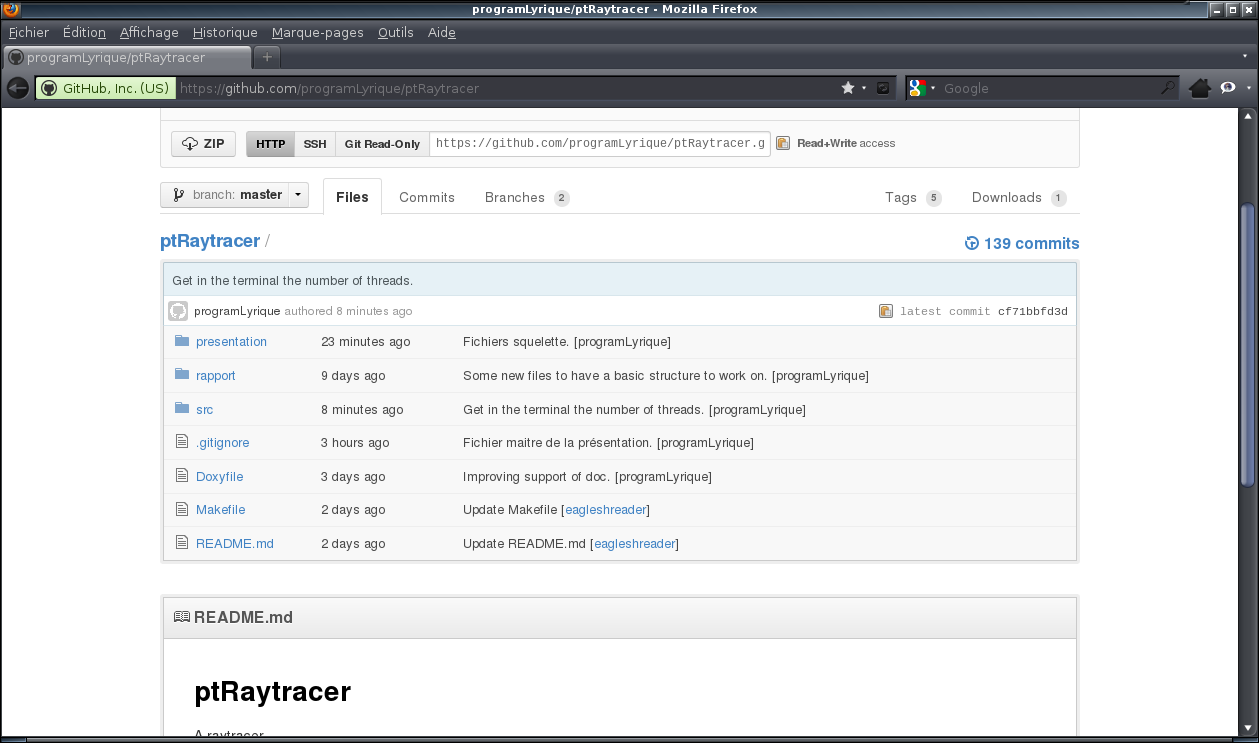
\includegraphics[scale=0.15]{Github.png}		
	\end{center}
	\caption{Page d'accueil du projet.} \label{Github}
	\end{figure}

  	\end{multicols}
\end{block}
}

\uncover<2->{
  \begin{block}{Branches}
  \only<2>{
  	\begin{figure}
  	\begin{center}
  		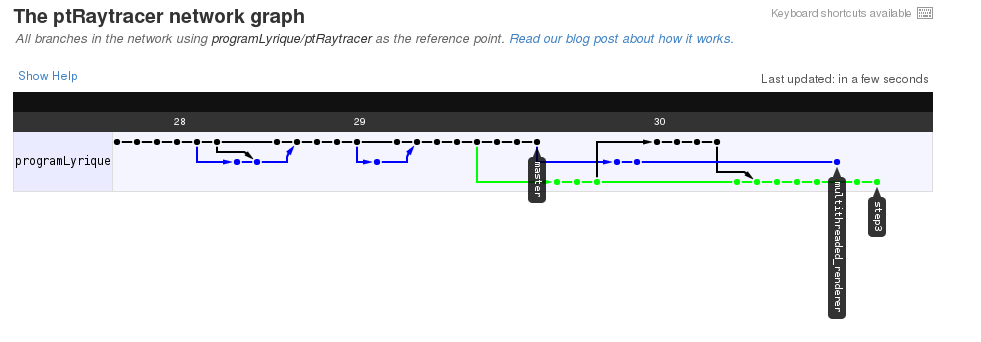
\includegraphics[scale=0.3]{arbreBranchesGit.png} 	
  	\end{center}
  	\caption{Les branches se séparent.} \label{Separent}
  	\end{figure}
	}
	\uncover<3>{	
	\begin{figure}
	\begin{center}
		  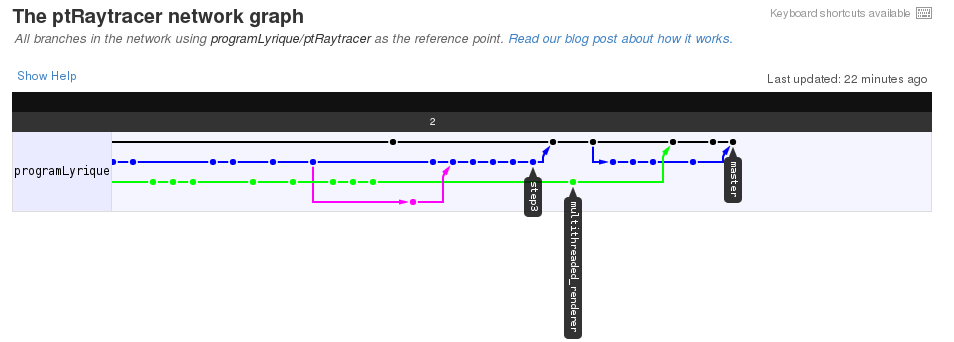
\includegraphics[scale=0.3]{arbreBranchesGit3.png}
	\end{center}
	\caption{Et se rejoignent.} \label{Rejoindre}
	\end{figure}
	}
  \end{block}
}
\end{frame}

\begin{frame}[fragile]
\frametitle{Documentation}
\framesubtitle{Doxygen}
\begin{verbatim}
/**
 * Renders a rectangle of the scene.
 * @param x x-coordinate of the left-upper vertex
 * @param y y-coordinate of the left-upper vertex
 * @param width width of the rectangle
 * @param height of the rectangle
 * @param oversampling if true, calculate 9 virtual pixels
 */
 void renderArea(int x, int y, int width, 
 	int height, screen& s, bool oversampling);
\end{verbatim}

\end{frame}

\begin{frame}{Principe du lancer de rayons}

\begin{itemize}
\item Lancer un rayon depuis la caméra, passant par un pixel de l'écran \footnote{Certaines techniques de lancer de rayons demandent un lancer de rayons depuis les lampes.}
\item Renvoyer le rayon vers les sources de lumière, en prenant en compte les éventuelles réflexions, et réfractions.
\item Prendre en compte la texture de l'objet (couleur, rugosité).
\item Combiner les informations de couleur.
\end{itemize}

\begin{center}
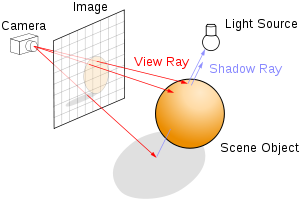
\includegraphics[scale=0.5]{raytracing.png}
\end{center}
\end{frame}



\begin{frame}
\frametitle{Hiérarchie de classes}

\begin{center}
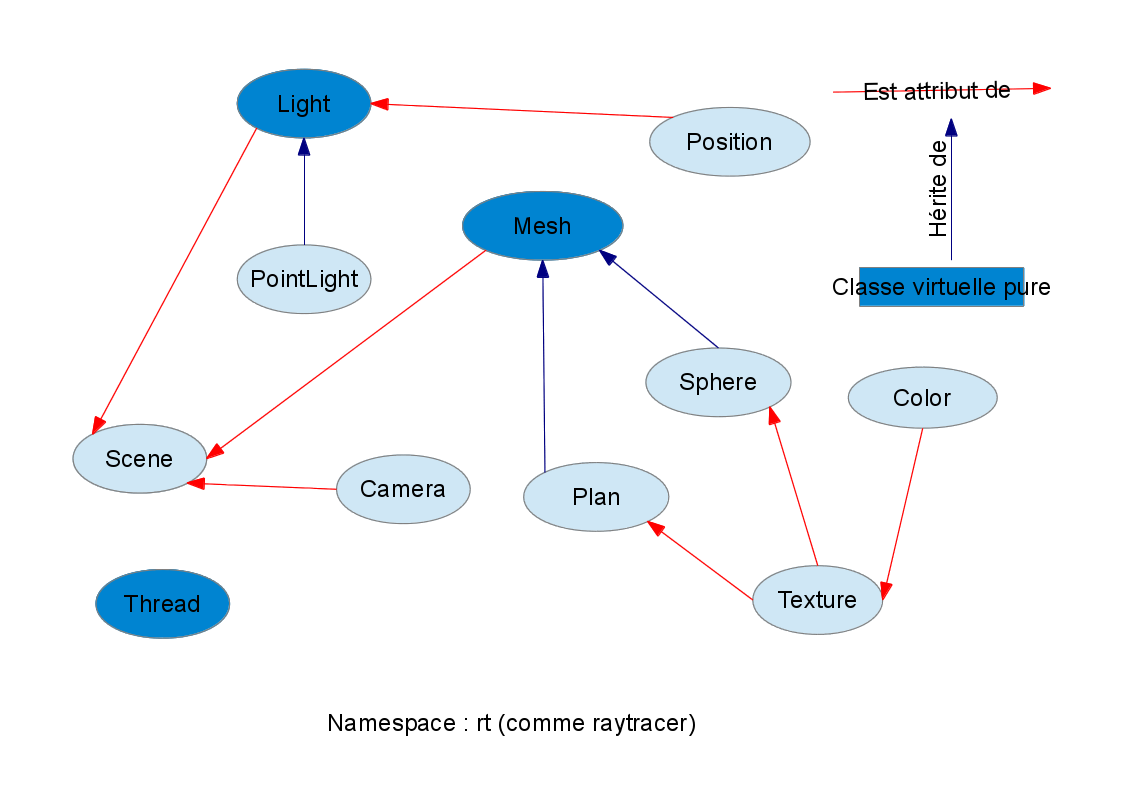
\includegraphics[scale=0.3]{hierarchie.png}
\end{center}

\end{frame}


\begin{frame}[fragile]
\frametitle{Créer des objets ou des lumières.}

\begin{block}{Objets}
Hériter de la classe Mesh, et implémenter :
\begin{verbatim}
 virtual bool intersect(const Position& pos, 
 	const vector& vect) = 0;
\end{verbatim}
\end{block}

\begin{block}{Lights}
Hériter de la classe Light, et implémenter :
\begin{verbatim}
virtual double illuminateR(const Position& position, 
	 const Mesh* m, const vector vision) = 0;
virtual double illuminateG(const Position& position, 
	const Mesh* m, const vector vision) = 0;
virtual double illuminateB(const Position& position, 
	const Mesh* m, const vector vision) = 0;
\end{verbatim}

\end{block}

Idem pour Camera.

\end{frame}

\begin{frame}[fragile]
\frametitle{Structures de données}

\begin{verbatim}
std::vector<Mesh*> objets;
std::vector<Light*> lights;

\end{verbatim}


\uncover<2->
{
	\begin{alertblock}{Inconvénients}
	Lors de la recherche d'une intersection, complexité linéaire en le nombre d'objets.
	Idem pour les lampes.
	\end{alertblock}
}

\uncover<3->
{
	\begin{block}{Des structures de données plus efficaces}
	Utiliser des octrees pour subdiviser l'espace, et effectuer l'intersection avec des noeuds ( « bounding boxes ») de l'arbre.
	\end{block}
}


\end{frame}

\begin{frame}
\frametitle{Caméra}

\begin{itemize}
\item Une caméra à la \emph{OpenGL} : oeil, direction de visée, vecteur selon la verticale
\item distance focale
\end{itemize}

\end{frame}





\section{Illumination}
\begin{frame}
	\frametitle{Illumination}
	\begin{block}{Comment faire?}
		Sphères affichées $\rightarrow$ gestion de la lumière qui se réfléchie sur les boules
	\end{block}
	\begin{block}{Illumination de Phong}
		\begin{enumerate}
			\item Lumière diffuse
			\item Lumière spéculaire
		\end{enumerate}
	\end{block}
\end{frame}
	
\begin{frame}
	\frametitle{Lumière diffuse}
	\begin{block}{Lumière diffuse}
		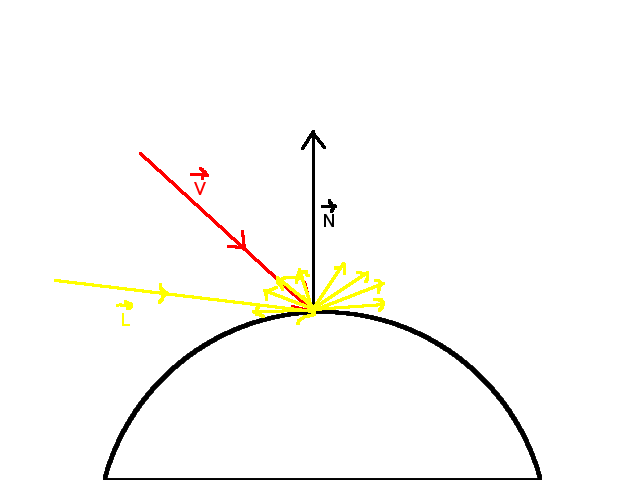
\includegraphics[width = 300px]{phong1.png} 
	\end{block}
\end{frame}
	
\begin{frame}
	\frametitle{Lumière spéculaire}
	\begin{block}{Lumière diffuse}
		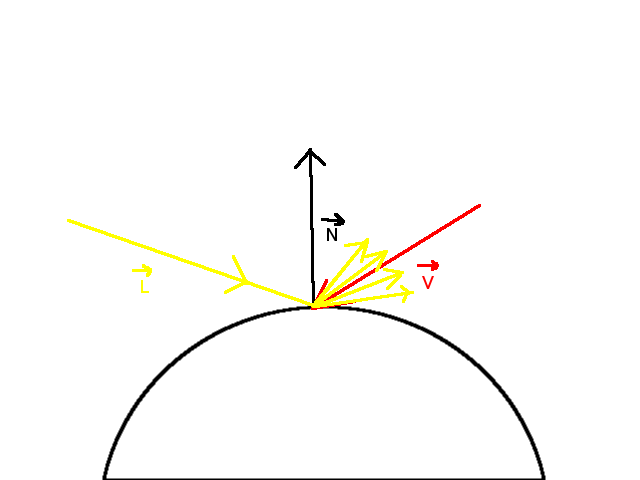
\includegraphics[width = 300px]{phong2.png} 
	\end{block}
\end{frame}

\begin{frame}
	\frametitle{Combinaison des 2}
	\begin{block}{Combinaison}
		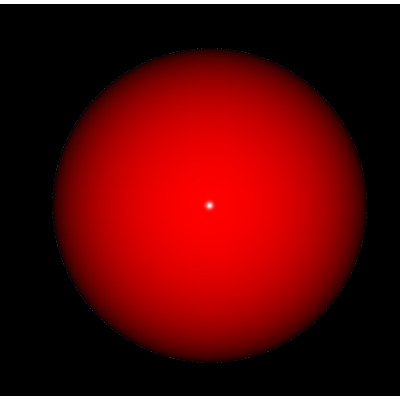
\includegraphics[width = 200px]{phong3.png} 
	\end{block}
\end{frame}

\begin{frame}
	\frametitle{Ajout de la réflexion}
	\begin{block}{Réflexion}
		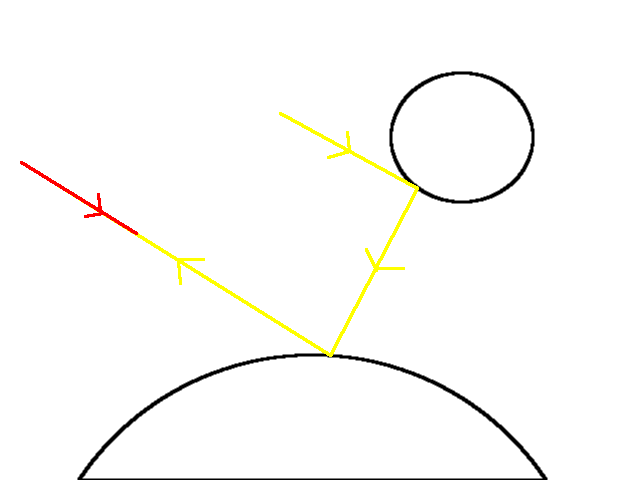
\includegraphics[width = 300px]{reflection.png} 
	\end{block}
\end{frame}

\begin{frame}
	\frametitle{Exemple de réflexion}
	\begin{block}{Exemple}
		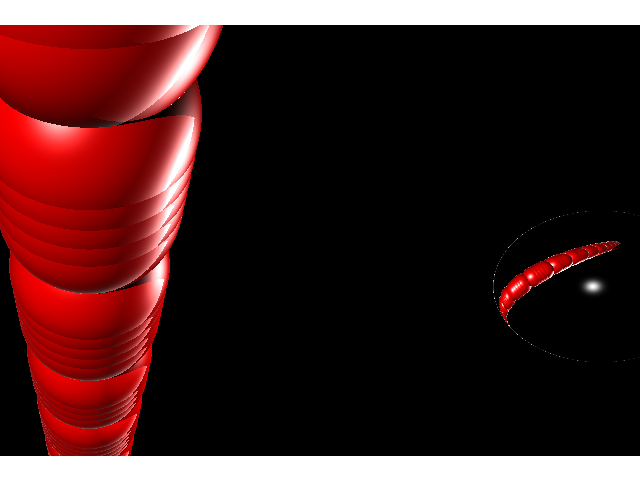
\includegraphics[width = 300px]{brillance.png} 
	\end{block}
\end{frame}

\begin{frame}
	\frametitle{Ajout de la transparence}
	\begin{block}{Transparence}
		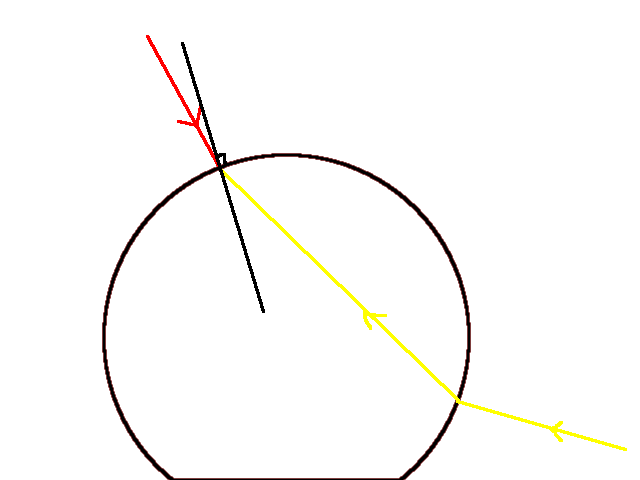
\includegraphics[width = 300px]{transparence.png} 
	\end{block}
\end{frame}

\begin{frame}
	\frametitle{Exemple de transparence}
	\begin{block}{Exemple}
		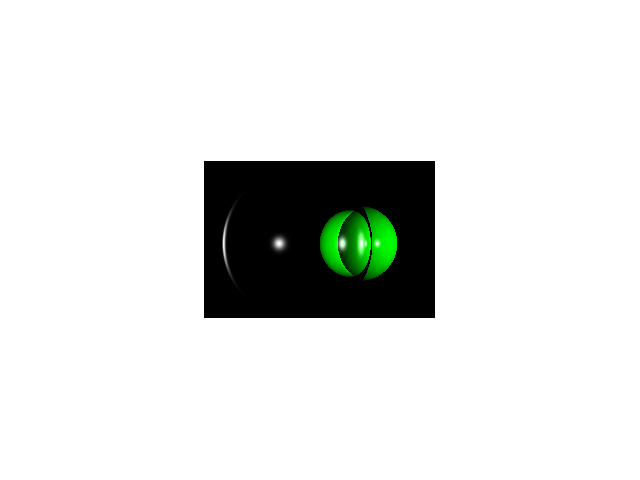
\includegraphics[width = 300px]{Untitled.png} 
	\end{block}
\end{frame}


\section{Multithreading} % Ou améliorations pour pouvoir caser l'anti-aliasing ?
\begin{frame}[fragile]
\frametitle{Threads}

\begin{block}{Posix threads}
Une bibliothèque de threads C : créer un \emph{wrapper} C++ pour être plus idiomatique.
\end{block}

\begin{block}{Utilisation du \emph{wrapper}}
Hériter de la classe Thread, et implémenter :
\begin{verbatim}
virtual void run() = 0;
\end{verbatim}
\end{block}

\end{frame}

\begin{frame}[fragile]
\frametitle{\emph{Wrapper}}
\begin{verbatim}
class Thread
{
    public:
        Thread();
        virtual ~Thread();
        pthread_t getHandle() const { return thread; }
        bool exec();
        bool join();
        static unsigned int nbCores();
    protected:
        virtual void run() = 0;
    private:
        pthread_t thread;
        static void * startRoutine(void * obj);
};
\end{verbatim}
\end{frame}


\begin{frame}
\frametitle{Parallélisation du lancer de rayon.}

\begin{block}{Facilement parallélisable}
Chaque pixel est rendu indépendamment des autres !
\end{block}

\begin{block}{Paralléliser}
\begin{itemize}
\item Détecter le nombre de coeurs.
\item Calcul du découpage\footnote{Oui, une puissance de 2 pour l'instant...} de l'image : $n \times m $ où $ n = \log_2(nbThreads) $ et $ m = nbThreads / n$.
\item Lancer un \emph{thread} par partie de l'image.
\end{itemize}
\end{block}

\end{frame}

\begin{frame}
\frametitle{Performances}
\begin{tabular}{|c|c|c|c|c|}
\hline 
Nombre de threads & 1 & 2 & 4 & 8 \\ 
\hline 
Temps (s) & 91 & 47 & 35 & 23 \\ 
\hline 
\end{tabular} 
\begin{block}{Banc de mesure}
\begin{tikzpicture}
\draw plot file {benchmark.txt};;
\end{tikzpicture}
\end{block}

\end{frame}

\begin{frame}
\frametitle{Améliorations}

\begin{itemize}
\item Découper l'image de façon adaptative.
\item Problèmes de synchronisation entre threads, et de conflit sur les données.
\end{itemize}
\end{frame}


%S'il j'ai eu le temps de l'implémenter
%\section{SBL}
%\input{sbl.tex}
\end{document}